\documentclass{article}
\usepackage[utf8]{inputenc}
%% Incluir gráficos
\usepackage{graphicx}
%% Incluir links entre páginas y contenidos %%
\usepackage{lastpage}
%% Nombres de figures, contents, referencias, etc. en español %%
\usepackage[spanish,es-tabla]{babel}
\usepackage{subcaption}
%% Para agregar lista de figuras y tablas de contenidos en el índice.
\usepackage{tocbibind}
%% Paquetes matemáticos
\usepackage{amsmath,amssymb,amsthm,textcomp}
\usepackage{glossaries} %% Glosarios
%% Figuras
\usepackage{float}
\usepackage{pythonhighlight}
\usepackage[margin=1in]{geometry}
\usepackage{color}
\usepackage{fancyvrb}
\usepackage{listings}
\usepackage{xcolor}

% useful packages
\usepackage[colorlinks=true, allcolors=blue]{hyperref}
\providecommand{\abs}[1]{\lvert#1\rvert}
\providecommand{\norm}[1]{\lVert#1\rVert}

%Nuevos comandos para definiciones, teoremas y cosas
\newtheorem{definicion}{Definición}
\newtheorem{teo}{Teorema}

% Para referencias 
%\usepackage[backend=biber, style=numeric, citestyle=numeric, sorting=nyt, maxcitenames=1, maxbibnames=99]{biblatex}
%\defbibheading{bibliography}[\refname]{}
%\addbibresource{bibliografia.bib}

\title{Informe de Práctica I, II y III}
\author{Lourdes Mella Miranda}
\date{Marzo 2024}

% Encabezados y pies de página personalizados %%------------------%
\usepackage{fancyhdr}
\pagestyle{fancy}
\lhead{}
\chead{}
\rhead{} %% \vspace*{-1cm}
\lfoot{}
\cfoot{}
\rfoot{Página \thepage\,de \pageref*{LastPage}}
\renewcommand{\headrulewidth}{0pt}
\renewcommand{\footrulewidth}{0pt}
\setlength{\parskip}{1em}

%-------------------------------------------------------------------------------------------------------------------------------------------------------------
\begin{document}
\begin{titlepage}
\begin{center}


\includegraphics[width=0.7\textwidth]{logo_usach.png}\\[1cm]


{\large Universidad de Santiago de Chile.}\\[0.5cm]
{\large Facultad de Ciencia.}\\[0.5cm]
{\large Departamento de Matemáticas y Ciencia de la Computación.}\\[0.5cm]

{\large Ingeniería Matemática.}\\[0.5cm]

% Title
\rule{\linewidth}{0.5mm} \\[0.4cm]
{ \huge \bfseries Informe de Práctica Profesional. \\[0.4cm] }
\rule{\linewidth}{0.5mm} \\[1.5cm]

% Author and supervisor
\noindent
\begin{minipage}{0.4\textwidth}
  \begin{flushleft} \large
  \end{flushleft}
\end{minipage}%
\begin{minipage}{0.4\textwidth}
  \begin{flushright} \large
    \emph{Estudiante:} \\
   Lourdes Mella Miranda
  \end{flushright}
\end{minipage}
\\

\vspace{1cm}

\noindent
\begin{minipage}{0.4\textwidth}
  \begin{flushleft} \large
  \end{flushleft}
\end{minipage}%
\begin{minipage}{0.4\textwidth}
  \begin{flushright} \large
    \emph{Profesor:} \\
   Rafael Labarca Briones
  \end{flushright}
\end{minipage}

\vfill

% Bottom of the page
{\large \today}
\end{center}
\end{titlepage}

%% Capítulos

\tableofcontents
%% \listoftables
%% \listoffigures
\newpage

\section{Información del practicante y la empresa.}
\subsection{Datos de la empresa.}

\begin{tabular}{r l}
    Razón social & EY SERVICIOS PROFESIONALES DE AUDITORIA Y ASESORIAS LIMITADA.\\
    Rut & 77.802.430-6.\\
	Tipo de Sociedad & Sociedad de responsabilidad limitada.\\
	Ubicación & Presidente Riesco 5435 piso 4, Las Condes, Santiago de Chile.\\

\end{tabular}

\subsection{Datos del practicante.}

\begin{tabular}{r l}
	Nombre & Lourdes Raquel del Pilar Mella Miranda.\\ 
	Rut & 20.055.740-9.\\
	Mail & lourdes.mella@usach.cl\\
	Institución & Universidad de Santiago de Chile.\\
	Facultad & Facultad de Ciencia.\\
	Departamento & Departamento de Matemática y Ciencia de la Computación.\\
	Carrera & Ingeniería Matemática.\\
	Tipo de práctica & Profesional.\\
	Cargo & Data Scientist practicante.\\
	Área & Consultoría\\
	Equipo & Digital Data \& Analytics.\\
	Supervisor & Loreto Sánchez\\
	Título supervisor & Ing. Civil Acústica, UACh.\\
	Postgrado supervisor & Candidata a Doctora en Ingeniería Eléctrica.

\end{tabular}

\section{Acerca de la empresa.}

\subsection{EY Chile}

Fundada en 2007, EY Chile es la filial chilena de Ernst \& Young (EY), una de las principales firmas de servicios profesionales a nivel mundial. Con una destacada presencia en el ámbito de la consultoría, auditoría, impuestos y asesoramiento financiero, EY Chile se ha consolidado como una entidad líder en el mercado. 

Recientemente, EY fue reconocida como la décima mejor empresa para trabajar en América Latina en 2023, según la lista de Great Place to Work. Este logro destaca el compromiso continuo de la firma con la calidad laboral y el bienestar de sus colaboradores. EY cuenta con una red global que abarca más de 700 ubicaciones en más de 150 países; asimismo, su filial chilena tiene presencia con oficinas estratégicas en Santiago, Viña del Mar, Concepción y Puerto Montt.

Para garantizar una atención especializada, EY Chile organiza sus servicios a través de diversas divisiones, brindando soluciones a una amplia gama de clientes. Estas divisiones incluyen:

\begin{itemize}

    \item \textbf{Estrategia y transacciones:} EY destaca en la prestación de servicios de estrategia y transacciones. Su enfoque personalizado a cada cliente, respaldado por una amplia experiencia multinacional, utiliza técnicas analíticas para impulsar decisiones de alto impacto. Esta firma se especializa en estrategia corporativa, asignación de capital y ejecución de transacciones, brindando apoyo a clientes de diversos sectores en la creación y preservación de valor. 

    \item \textbf{Consultoría:} La consultoría en EY impulsa la transformación empresarial al integrar estratégicamente personas, tecnología e innovación. Adaptándose a la rápida evolución del entorno laboral, la firma fomenta comportamientos innovadores y colaborativos para abordar desafíos clave en la actualidad. Al priorizar a las personas, aprovechar la tecnología de manera ágil y promover la innovación, EY genera valor a largo plazo para individuos, empresas y la sociedad en general.

    \item \textbf{Auditoría y finanzas:} Los equipos de Auditoría y Finanzas de EY en Chile desempeñan un papel crucial al servir al interés público, promoviendo la confianza en empresas y mercados de capitales. A través de servicios que abarcan auditoría, asesoría en contabilidad financiera y análisis forense, EY aborda riesgos, complejidades y oportunidades, protegiendo y promoviendo un valor sostenible a largo plazo.

    \item \textbf{Impuestos:} Los profesionales de impuestos de EY en Chile ofrecen servicios completos en todas las disciplinas tributarias. Con competencias en impuestos empresariales, internacionales, sobre transacciones y legislación, EY combina conocimiento y experiencia para ayudar a las empresas a prosperar en un entorno de cambios rápidos.

    \item \textbf{EY Law - Servicios legales:} EY Law proporciona orientación detallada para abordar el complejo entorno legal global. Con un enfoque multidisciplinario, la firma ayuda a reducir la brecha entre asesores de negocios y legales, aumentando la eficiencia y velocidad de comercialización. Su enfoque centrado en el sector brinda asesoría integrada y detallada, con servicios gestionados de manera centralizada para empresas en todo el mundo.
    
    \end{itemize}

\subsection{Visión general.}

\begin{itemize}
\item[\textbf{Misión:}] ``Construir un mejor mundo de negocios mediante servicios de calidad que fomentan la confianza en los mercados y el desarrollo de líderes excepcionales.''

\item[\textbf{Visión:}] ``En EY, estamos construyendo el lugar de trabajo del futuro, más inteligente, inclusivo y dinámico, adaptándonos al cambio y promoviendo el crecimiento económico más inclusivo.''

\item[\textbf{Valores:}] 

\begin{enumerate}
    
    \item[i)] \emph{Integridad:} ``Demostramos honestidad y coherencia en todas nuestras acciones y decisiones.''  
    \item[ii)] \emph{Respeto:} ``Valoramos y reconocemos las diferencias individuales, fomentando un ambiente inclusivo y de respeto mutuo.'' 
    \item[iii)] \emph{Trabajo en equipo:} ``Colaboramos de manera efectiva, reconociendo la importancia del trabajo conjunto para lograr el éxito.''
    \item[iv)] \emph{Inclusión:} ``Valoramos y potenciamos las diferencias individuales, reconociendo que la diversidad impulsa la innovación y contribuye al éxito a largo plazo en el mercado global.''
    \item[v)] \emph{Energía:}  ``Demostramos vitalidad y pasión en nuestra labor diaria, buscando continuamente formas de agregar valor.''
    \item[vi)] \emph{Entusiasmo:} ``Mostramos un entusiasmo positivo hacia nuestros colegas, clientes y desafíos profesionales.''
    \item[vii)] \emph{Coraje para liderar:}  ``Nos destacamos por asumir la responsabilidad y liderar con valentía, basándonos en principios éticos y en hacer lo correcto en nuestras relaciones.''
   
\end{enumerate}

\item[\textbf{Logo:}]
\end{itemize}

\begin{center}
    
\includegraphics[scale=0.2]{EY_logo.png}
\end{center}

\section{Aspectos generales y contextualización}

\subsection{Marco conceptual}

La industria ha experimentado una evolución constante, desde sus primeras etapas hasta la revolución actual de la Industria 4.0. Cada fase ha marcado un hito en el desarrollo de nuevas tecnologías y enfoques de producción, llevándonos a la actual convergencia de tecnologías digitales. A continuación, presentamos una ilustración que representa la evolución industrial a lo largo del tiempo.

\begin{center}
\begin{figure}[h]
  \centering
  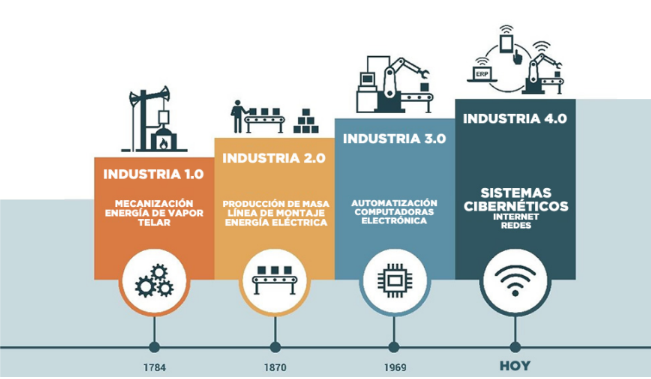
\includegraphics[width=0.8\textwidth]{industria.png}
  \caption{Evolución Industrial}
\end{figure}    
\end{center}

Hoy en día, nos encontramos inmersos en la era de la Industria 4.0, una revolución industrial impulsada por el impacto de la tecnología digital y el procesamiento avanzado de datos. Este cambio de paradigma ha dado origen a las denominadas fábricas inteligentes, redefiniendo por completo los modelos de producción y generando una creciente automatización que impulsa la productividad a niveles sin precedentes.

En esta nueva era industrial, es crucial comprender conceptos clave que impulsan la transformación. Definamos algunos de estos términos fundamentales:

\begin{itemize}

    \item \textbf{Internet de las Cosas (IoT):} Se refiere a la interconexión de dispositivos y sistemas a través de la red, permitiendo la recopilación y el intercambio de datos en tiempo real. El IoT es un componente esencial para la operación eficiente de fábricas inteligentes.

    \item \textbf{Big Data:} Aborda la gestión y análisis de conjuntos de datos masivos. En la Industria 4.0, el Big Data juega un papel crucial al procesar la gran cantidad de información generada por sensores y dispositivos conectados, proporcionando conclusiones valiosas para la toma de decisiones. 
  
    \item \textbf{Cloud computing:} La computación en la nube ofrece almacenamiento y procesamiento de datos de forma remota, permitiendo el acceso a recursos computacionales escalables. De este modo, se facilita la gestión eficiente de grandes cantidades de datos y servicios.
    
\end{itemize}

En el ámbito industrial, la gestión del mantenimiento se ha transformado significativamente debido al desarrollo tecnológico de los equipos de control y medida. A continuación definimos los tres principales tipos de mantenimiento:

\begin{itemize}
    \item \textbf{Mantenimiento Correctivo:} Actúa tras la ocurrencia de una avería, minimizando tiempos de detención de maquinaria. Sin embargo, puede generar tiempos muertos no planificados.

    \item \textbf{Mantenimiento Preventivo:} Realiza ajustes programados para mantener herramientas y equipos en condiciones seguras. Aunque permite una planificación anticipada, puede dar lugar a intervenciones innecesarias y costos constantes.

    \item \textbf{Mantenimiento Predictivo:} Evalúa el estado de la maquinaria en tiempo real basándose en su condición. Utiliza sensores para recopilar datos, luego procesa esta información para determinar la necesidad de intervención. Logra optimizar la fiabilidad y disponibilidad de la maquinaria a un costo mínimo.
    
\end{itemize}

\begin{center}
\begin{figure}[h]
  \centering
  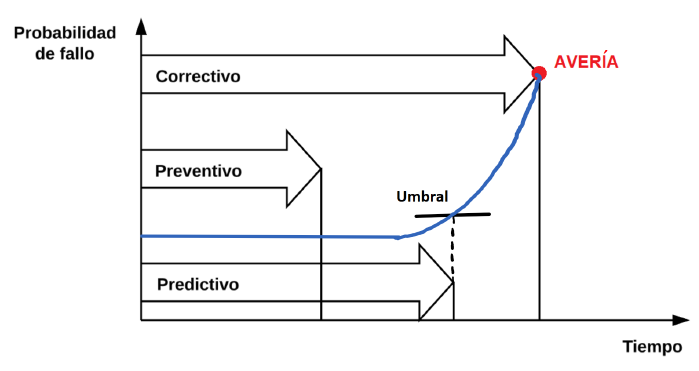
\includegraphics[width=0.7\textwidth]{mantenimiento.png}
  \caption{Tipos de mantenimiento}
\end{figure}    
\end{center}

Con lo expuesto anteriormente, se evidencia la estrecha relación entre el mantenimiento predictivo y la Industria 4.0. Este enfoque de mantenimiento, al evaluar en tiempo real el estado de la maquinaria basándose en datos recopilados por sensores, se alinea perfectamente con la interconexión de dispositivos propuesta por el Internet de las Cosas (IoT). Sin duda, la capacidad de recopilar, procesar y analizar grandes conjuntos de datos, conocida como Big Data, se convierte en un pilar fundamental para el éxito del mantenimiento predictivo. Además, la adopción de tecnologías como la computación en la nube (Cloud Computing) potencia la eficiencia operativa al proporcionar un entorno escalable y accesible para el procesamiento de datos.

\subsection{Contexto}

El equipo de Digital Data \& Analytics donde realicé mi práctica profesional,

\end{document}
